\section{Probing}%
\label{sec:probing}

\begin{frame}
	\frametitle{Probing}
	\begin{center}
		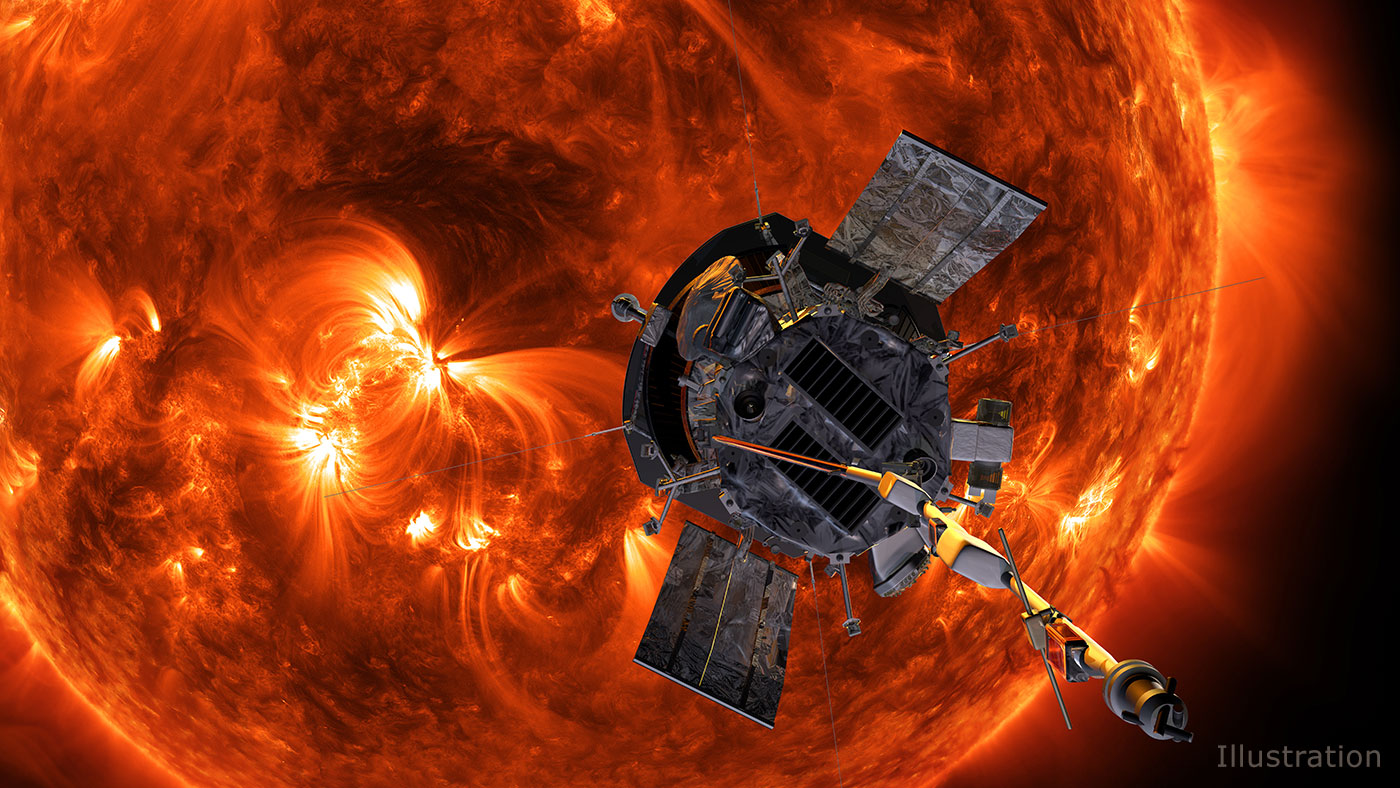
\includegraphics[width=0.8\textwidth]{figures/probe.jpg}\\
		\hspace*{15pt}\hbox{\scriptsize Image By:\thinspace{\itshape NASA/Johns Hopkins APL/Steve Gribben }}
		% https://www.jpl.nasa.gov/news/news.php?feature=7224
	\end{center}
\end{frame}

\begin{frame}
	\frametitle{Probing}
		\begin{block}{Linear Probing}
			If an entry is already taken, move on to the next available entry in the table.\\
			Harder to implement (as we we will soon see), but no extra space required for linked lists!
		\end{block}	
		\pause
		\begin{questionblock}{Quick practice}
		  Take hash function $f(k) = 2k + 3$ and a map of \textit{fixed} size $10$. What does a map look like that has the
			keys: $1,2,7,12,13,19,22,27$?
		\end{questionblock}
		\pause
		\begin{answerblock}{Lets draw it}
			We have a smart board available.
		\end{answerblock}
\end{frame}

\begin{frame}
	\frametitle{Hang on...}

	\begin{questionblock}{What about retrieving items}
		What happens when we now retrieve an item?	\\
		For instance what happens when we want to get key 22 back from the map?
	\end{questionblock}
	\pause
	\begin{answerblock}{Keep on walking, keep on walking}
		We start at the hash and walk until we find the value or an \alert<3->{empty place}.
	\end{answerblock}
	\pause
	\begin{problemblock}{Deleting in the middle}	
		But what if before that key 19 had been deleted?
	\end{problemblock}
\end{frame}

\begin{frame}
	\frametitle{Deleting keys}
	\begin{questionblock}{What to do, what to do?}
		How should we handle deletions?
		\begin{enumerate}[A.]
			\item Set the index to \texttt{None}.
			\item Set the index to some special marker.
			\item Check the rest of the items and move them back 1 if their hash demands it.
			\item Rebuild the whole map.
		\end{enumerate}
	\end{questionblock}
	\pause
	\begin{answerblock}{A defunct marker}
    We mark the entry as \textit{defunct}.\\
		Meaning: an item was once here, but it can now be reused.		
	\end{answerblock}
\end{frame}

\begin{frame}
	\frametitle{So to find an item...}
	
\end{frame}

\begin{frame}
	\frametitle{In Python}
	\lstinputlisting{code/probing.py}
\end{frame}

\begin{frame}
	\frametitle{But hang on...}
	\framesubtitle{Again!}

	\vspace{-5pt}
	\lstinputlisting[firstline=3, lastline=7]{code/probing.py}
	\vspace{-5pt}
	\begin{questionblock}{I'm stuffed}
		What happens when the map is completely full?\\
		\vspace{-5pt}
		\begin{enumerate}[A.]
			\item We never find an empty cell and loop forever.
			\item The list is at most 50\% full at all times.
			\item The last entry of the list is always empty.
			\item I don't know.
		\end{enumerate}
	\end{questionblock}
	\pause
		\vspace{-5pt}
	\begin{answerblock}{Keep on walking, keep on walking}
		Remember that as soon as we had the risk of being half full, we resized the map. This ensures there are always some
		None places.
	\end{answerblock}
\end{frame}
